\documentclass{article}
% main document, called main.tex
\usepackage{amsmath,amssymb}
\usepackage{tikz}
\usetikzlibrary{shapes}
\usepackage{pgfplots}
\usetikzlibrary{calc}
\usetikzlibrary{matrix,arrows,patterns.meta}
\usepackage{graphicx}
\usetikzlibrary{external}
\tikzexternalize[shell escape=-enable-write18,prefix=figures/]
% activate

%\tikzset{external/system call={latex \tikzexternalcheckshellescape -halt-on-error -interaction=batchmode -jobname "\image" "\texsource"; dvips -o "\image".ps "\image".dvi}}


\begin{document}
	
\tikzsetnextfilename{test}
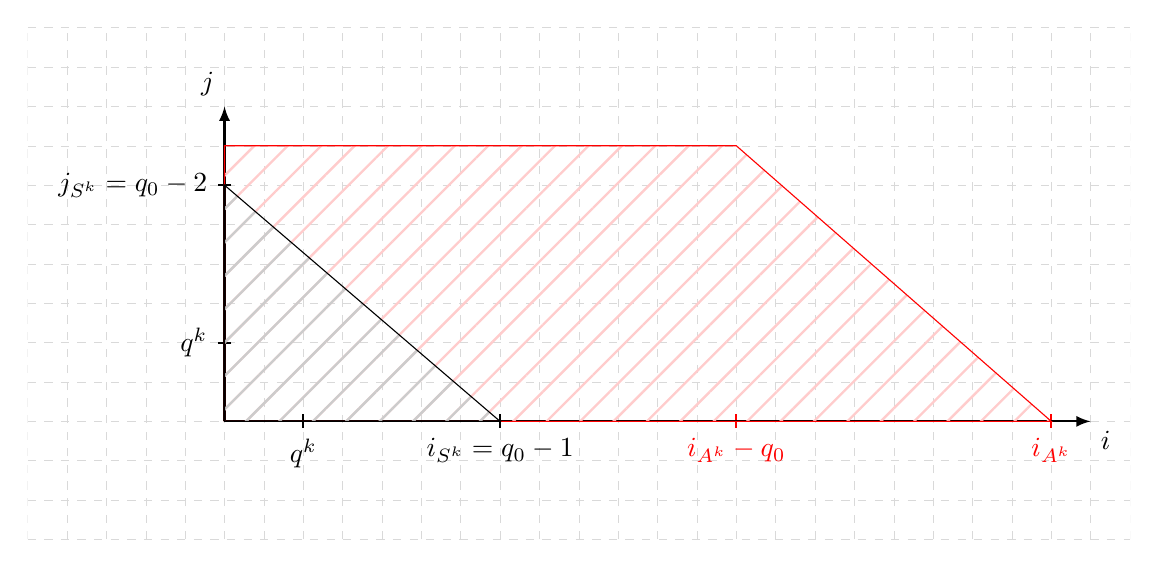
\begin{tikzpicture}[scale=0.5]
	\def\qO{8};
	\def\q{2};
	\def\iAk{21};
	\def\largeur{\iAk+2}
	\def\hauteur{\qO+2}
\clip (-5,-3) rectangle (\largeur,\hauteur); % Clips the picture...
\draw[style=help lines,dashed,opacity=0.3] (-5,-3) grid[step=1cm] (\largeur,\hauteur); % Draws a grid in the new coordinates.

%Sommets des polygones
\coordinate (A) at (\iAk,0) {};
\coordinate (B) at (\iAk-\qO,\qO-1) {};
\coordinate (C) at (0,\qO-1) {};
\coordinate (D) at (0,\qO-2) {};
\coordinate (E) at (\qO-1,0) {} ;

%Marqueurs sur l'axe vertical
\draw[thick] (5pt,\q) -- (-5pt,\q) node[anchor=east] {$q^k$} ;
\draw[thick] (5pt,\qO-2) -- (-5pt,\qO-2) node[anchor=east] {$j_{S^k}=q_0-2$} ;


%Marqueurs sur l'axe horizontal
\draw[thick,red] (\iAk-\qO,5pt) -- (\iAk-\qO,-5pt) node[anchor=north] {$i_{A^k}-q_ 0$} ;
\draw[thick,red] (\iAk,5pt) -- (\iAk,-5pt) node[anchor=north] {$i_{A^k}$} ;
\draw[thick] (\q,5pt) -- (\q,-5pt) node[anchor=north] {$q^k$} ;
\draw[thick] (\qO-1,5pt) -- (\qO-1,-5pt) node[anchor=north] {$i_{S^k}=q_0-1$} ;



%Axes
\draw [thick,-latex] (0,0) -- (0,\qO) node [above left] {$j$};
\draw [thick,-latex] (0,0) -- (\iAk+1,0) node [below right] {$i$};

%Formes
\filldraw [ pattern color=red!20,
	pattern={Lines[
	distance=3mm,
	angle=45,
	line width=0.3mm]},
	draw=red] (0,0) -- (A) -- (B) -- (C) -- cycle;

\filldraw [ pattern color=black!20,
pattern={Lines[
	distance=3mm,
	angle=45,
	line width=0.3mm]},
draw=black] (0,0) -- (E) -- (D)-- cycle;


 
\end{tikzpicture} 



\end{document}